% -*- mode: noweb; noweb-default-code-mode: R-mode; -*-
\documentclass[a4paper]{article}

\title{A Test File}
\author{Friedrich Leisch}


\usepackage{a4wide}

\usepackage{Sweave}
\begin{document}

\maketitle

A simple example: the integers from 1 to 10 are
\begin{Schunk}
\begin{Soutput}
 [1]  1  2  3  4  5  6  7  8  9 10
\end{Soutput}
\end{Schunk}

We can also emulate a simple calculator:
\begin{Schunk}
\begin{Sinput}
> 1 + 1
\end{Sinput}
\begin{Soutput}
[1] 2
\end{Soutput}
\begin{Sinput}
> 1 + pi
\end{Sinput}
\begin{Soutput}
[1] 4.141593
\end{Soutput}
\begin{Sinput}
> sin(pi/2)
\end{Sinput}
\begin{Soutput}
[1] 1
\end{Soutput}
\end{Schunk}

Now we look at Gaussian data:

\begin{Schunk}
\begin{Soutput}
 [1]  0.89537546 -0.42302093  1.38415521 -1.17404139 -0.11382677 -0.10022515 -0.45769241 -0.35709716
 [9] -1.05509226 -0.07186432 -2.06506074 -0.05614488 -0.22260512 -1.19194086 -1.28036594  1.05782122
[17]  0.64618955  1.61105441  0.10580153 -0.64133647
\end{Soutput}
\begin{Soutput}
	One Sample t-test

data:  x
t = -0.82804, df = 19, p-value = 0.4179
alternative hypothesis: true mean is not equal to 0
95 percent confidence interval:
 -0.6190920  0.2681003
sample estimates:
 mean of x 
-0.1754959 
\end{Soutput}
\end{Schunk}
Note that we can easily integrate some numbers into standard text: The
third element of vector \texttt{x} is 1.38415521013093, the
$p$-value of the test is 0.41793. % $

Now we look at a summary of the famous \texttt{iris} data set, and we
want to see the commands in the code chunks:



\begin{Schunk}
\begin{Sinput}
> data(iris)
> summary(iris)
\end{Sinput}
\begin{Soutput}
  Sepal.Length    Sepal.Width     Petal.Length    Petal.Width          Species  
 Min.   :4.300   Min.   :2.000   Min.   :1.000   Min.   :0.100   setosa    :50  
 1st Qu.:5.100   1st Qu.:2.800   1st Qu.:1.600   1st Qu.:0.300   versicolor:50  
 Median :5.800   Median :3.000   Median :4.350   Median :1.300   virginica :50  
 Mean   :5.843   Mean   :3.057   Mean   :3.758   Mean   :1.199                  
 3rd Qu.:6.400   3rd Qu.:3.300   3rd Qu.:5.100   3rd Qu.:1.800                  
 Max.   :7.900   Max.   :4.400   Max.   :6.900   Max.   :2.500                  
\end{Soutput}
\end{Schunk}


\begin{figure}[htbp]
  \begin{center}
\begin{Schunk}
\begin{Sinput}
> library(graphics)
> pairs(iris)
\end{Sinput}
\end{Schunk}
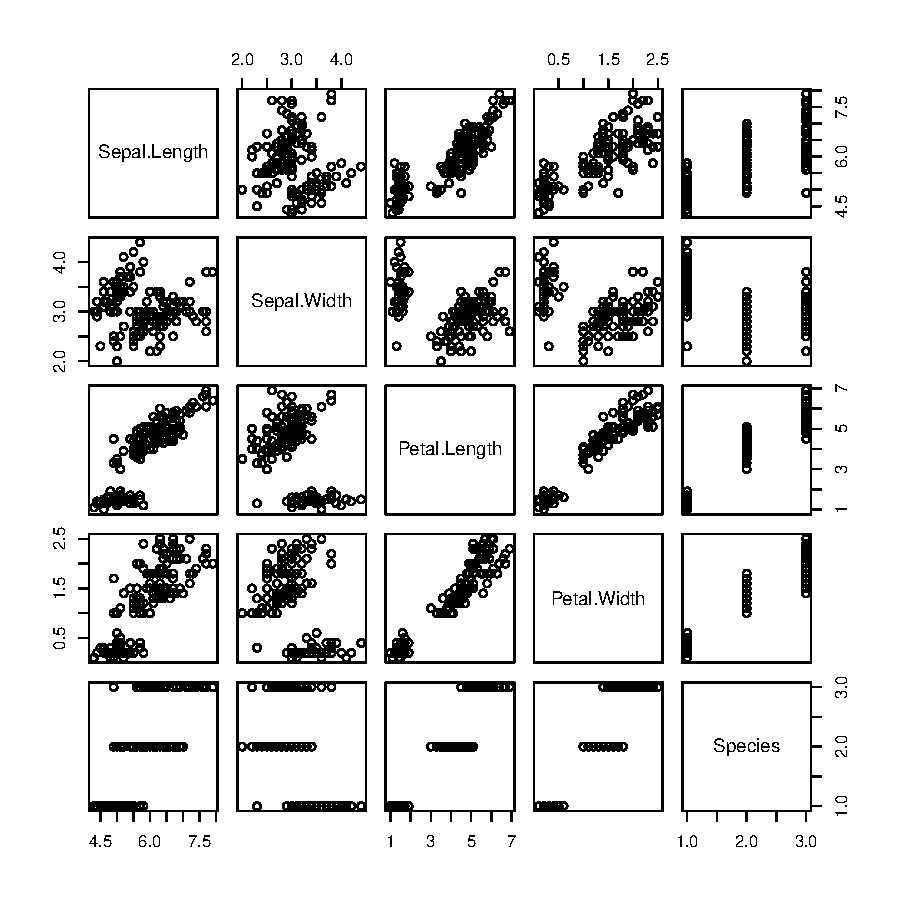
\includegraphics{Sweave-test-1-006}
     \caption{Pairs plot of the iris data.}
  \end{center}
\end{figure}

\begin{figure}[htbp]
  \begin{center}
\begin{Schunk}
\begin{Sinput}
> boxplot(Sepal.Length~Species, data=iris)
\end{Sinput}
\end{Schunk}
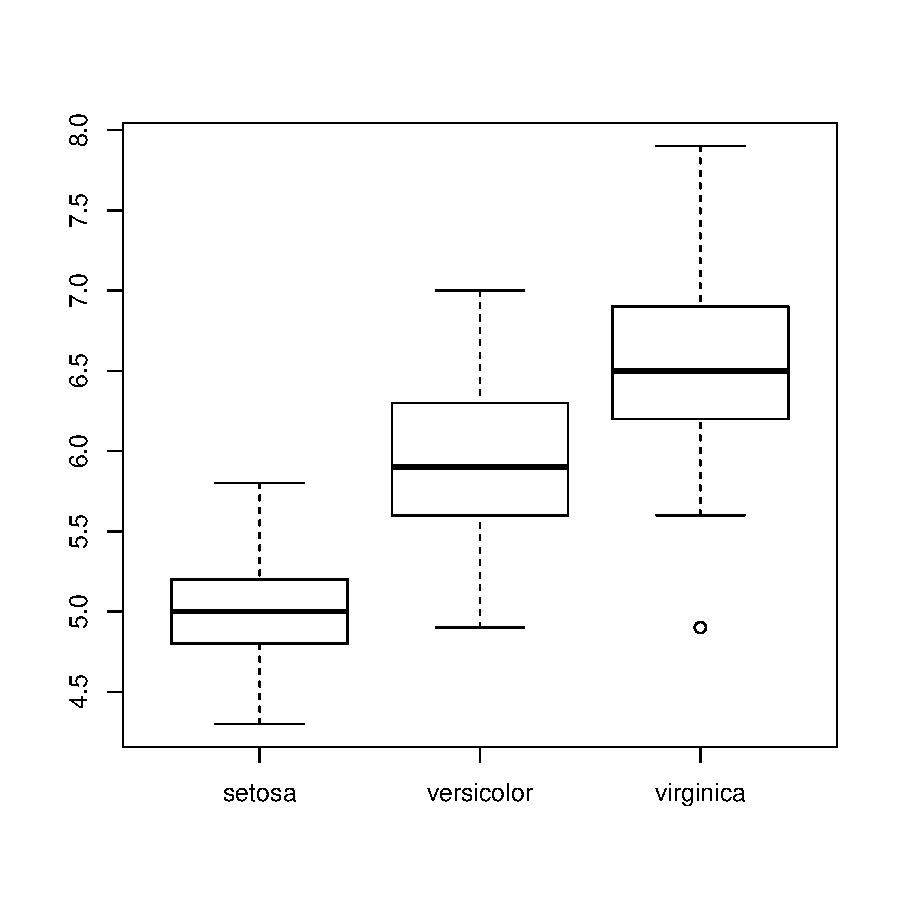
\includegraphics{Sweave-test-1-007}
    \caption{Boxplot of sepal length grouped by species.}
  \end{center}
\end{figure}

\end{document}
